\documentclass[../AnalysisNoteJBuxton.tex]{subfiles}
\begin{document}

\subsubsection{Results: \texorpdfstring{$\Lambda$K$^{0}_{S}$ and $\Lambda$K$^{\pm}$: 10 Residual Correlations Included in Fit}{TEXT}}
\label{ResultsLamK_10Res}

\begin{figure}[h]
  \centering
  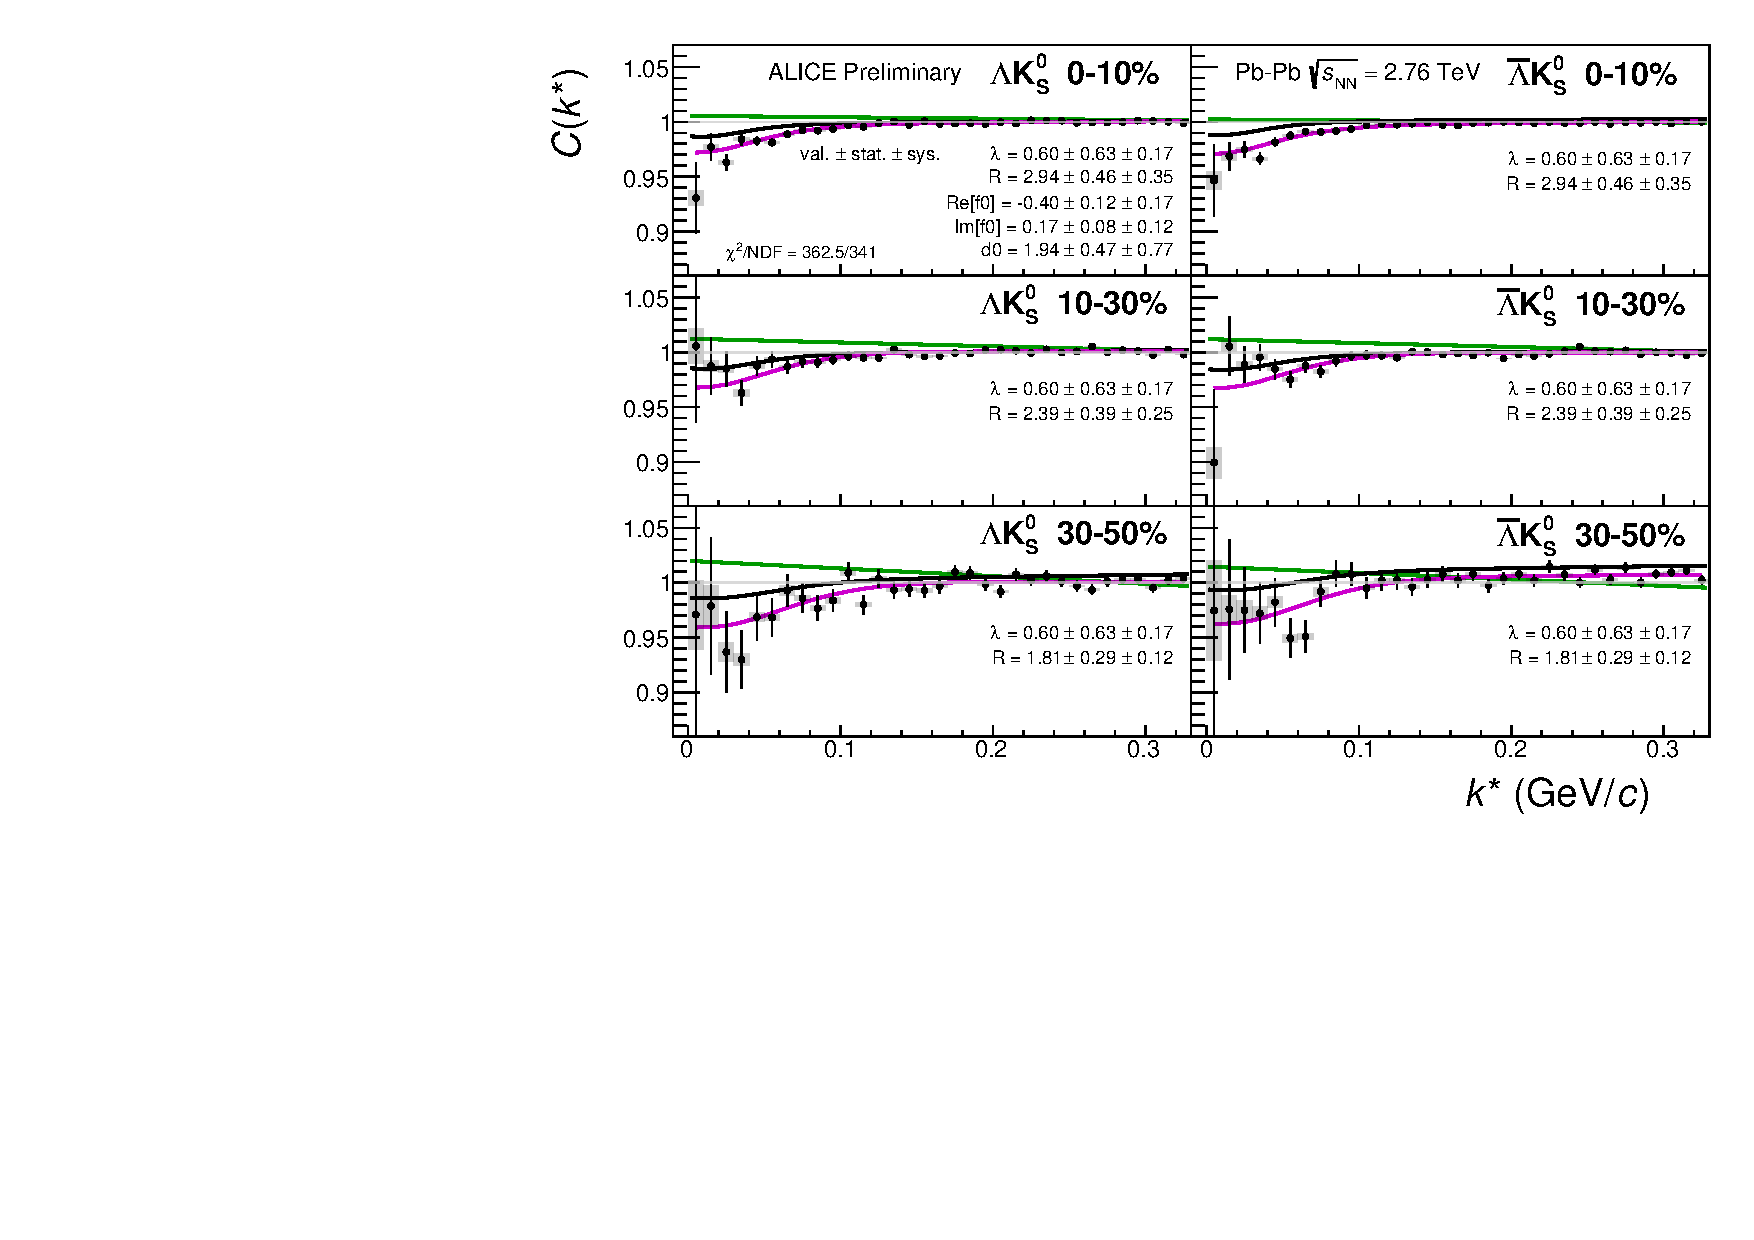
\includegraphics[width=\textwidth]{7_ResultsAndDiscussion/Figures/canKStarCfwFitsLamK0wConj_0010_1030_3050_MomResCrctn_NonFlatBgdCrctn_SingleLamParam_10Res_PrimMaxDecay4fm_UsingXiDataAndCoulombOnly.pdf}
  \caption[$\Lambda$K$^{0}_{S}$($\bar{\Lambda}$K$^{0}_{S}$) Fits with 10 Residuals]{Fits, with 10 residual correlations included, to the $\Lambda$K$^{0}_{S}$ (left) and $\bar{\Lambda}$K$^{0}_{S}$ (right) data for the centralities 0-10\% (top), 10-30\% (middle), and 30-50\% (bottom).
The lines represent the statistical errors, while the boxes represent the systematic errors.
Each has unique $\lambda$ and normalization parameters.
The radii are shared amongst like centralities; the scattering parameters ($\mathbb{R}f_{0}$, $\mathbb{I}f_{0}$, $d_{0}$) are shared amongst all.
The black solid line represents the ``raw" fit, i.e. not corrected for momentum resolution effects nor non-flat background.  
The green line shows the fit to the non-flat background.
The purple points show the fit after momentum resolution and non-flat background corrections have been applied.
The initial values of the parameters is listed, as well as the final fit values with uncertainties.
Here, $R$ was restricted to [2.,10.] and $\Lambda$ was restricted to [0.1,0.8].}
  \label{fig:LamK0wConjFits_10Res}
\end{figure}

\begin{comment}
\begin{figure}[h]
  \centering
  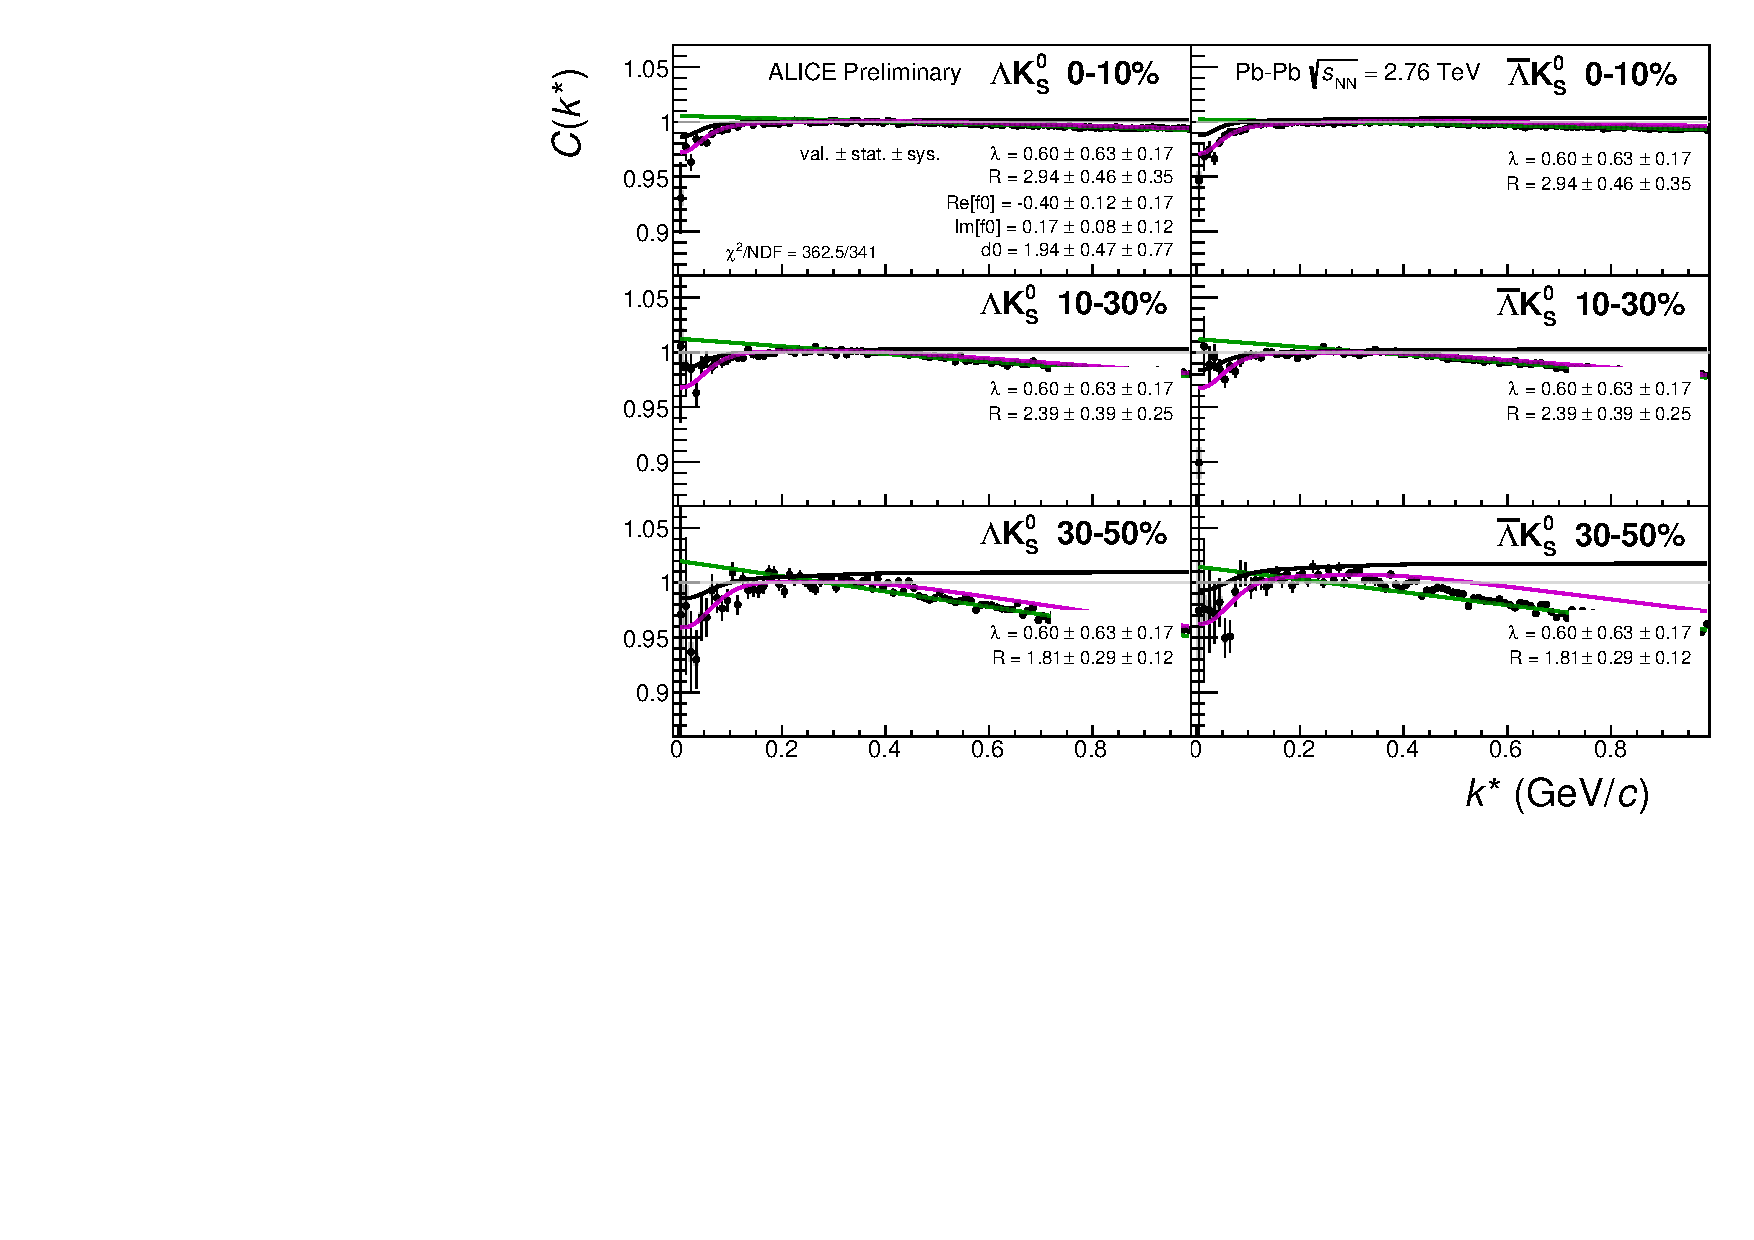
\includegraphics[width=\textwidth]{7_ResultsAndDiscussion/Figures/canKStarCfwFitsLamK0wConj_0010_1030_3050UnZoomed_MomResCrctn_NonFlatBgdCrctn_SingleLamParam_10Res_PrimMaxDecay4fm_UsingXiDataAndCoulombOnly.pdf}
  \caption[$\Lambda$K$^{0}_{S}$($\bar{\Lambda}$K$^{0}_{S}$) Fits with 10 Residuals (Wide Range)]{Same as Fig. \ref{fig:LamK0wConjFits_10Res}, but with a wider range of view.  
Fits, with 10 residual correlations included, to the $\Lambda$K$^{0}_{S}$ (left) and $\bar{\Lambda}$K$^{0}_{S}$ (right) data for the centralities 0-10\% (top), 10-30\% (middle), and 30-50\% (bottom).
The lines represent the statistical errors, while the boxes represent the systematic errors.
Each has unique $\lambda$ and normalization parameters.
The radii are shared amongst like centralities; the scattering parameters ($\mathbb{R}f_{0}$, $\mathbb{I}f_{0}$, $d_{0}$) are shared amongst all.
The black solid line represents the ``raw" fit, i.e. not corrected for momentum resolution effects nor non-flat background.  
The green line shows the fit to the non-flat background.
The purple points show the fit after momentum resolution and non-flat background corrections have been applied.
The initial values of the parameters is listed, as well as the final fit values with uncertainties.
Here, $R$ was restricted to [2.,10.] and $\Lambda$ was restricted to [0.1,0.8].}
  \label{fig:LamK0wConjFitsUnZoomed_10Res}
\end{figure}
\end{comment}



\begin{figure}[h]
  \centering
  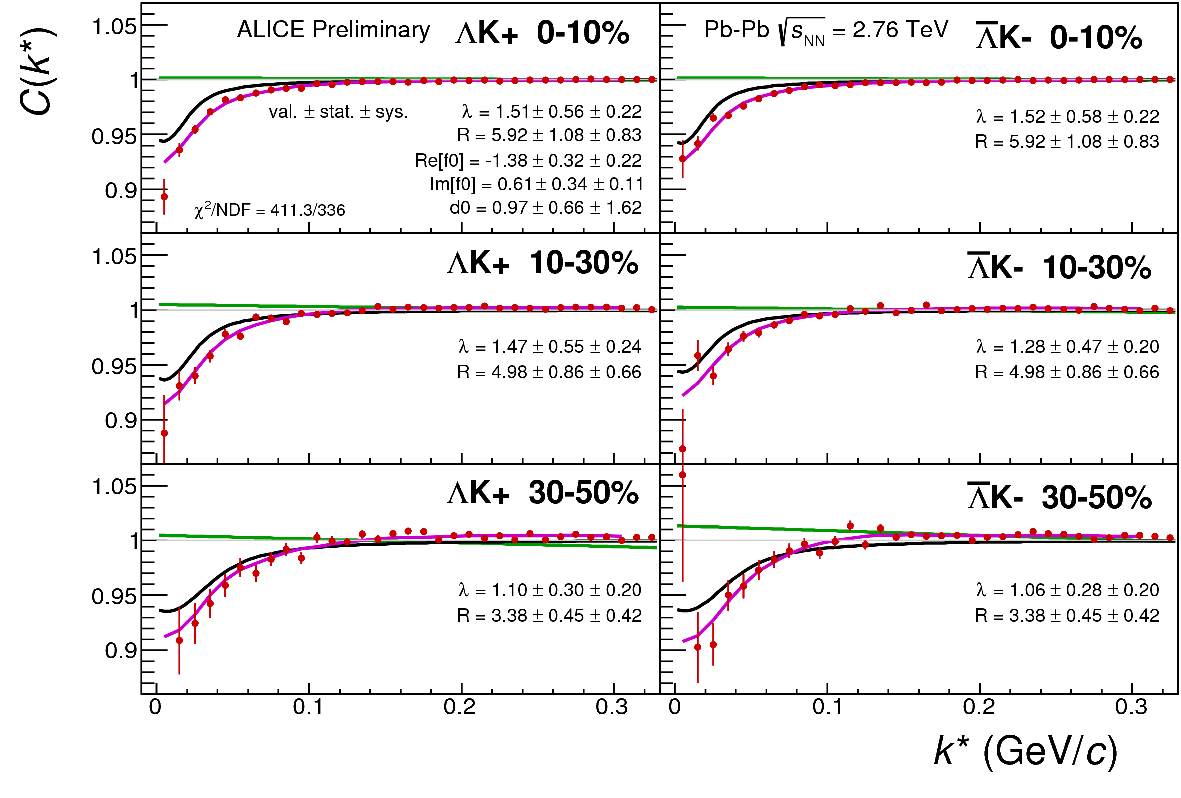
\includegraphics[width=\textwidth]{7_ResultsAndDiscussion/Figures/canKStarCfwFitsLamKchPwConj_0010_1030_3050_MomResCrctn_NonFlatBgdCrctn_10Res_PrimMaxDecay4fm_UsingXiDataAndCoulombOnly.pdf}
  \caption[$\Lambda$K$^{+}$($\bar{\Lambda}$K$^{-}$) Fits with 10 Residuals]{Fits, with 10 residual correlations included, to the $\Lambda$K$^{+}$ (left) and $\bar{\Lambda}$K$^{-}$ (right) data for the centralities 0-10\% (top), 10-30\% (middle), and 30-50\% (bottom).
The lines represent the statistical errors, while the boxes represent the systematic errors.  
Each has unique $\lambda$ and normalization parameters.
The radii are shared amongst like centralities; the scattering parameters ($\mathbb{R}f_{0}$, $\mathbb{I}f_{0}$, $d_{0}$) are shared amongst all.
The black solid line represents the ``raw" fit, i.e. not corrected for momentum resolution effects nor non-flat background.  
The green line shows the fit to the non-flat background.
The purple points show the fit after momentum resolution and non-flat background corrections have been applied.
The initial values of the parameters is listed, as well as the final fit values with uncertainties.}
  \label{fig:LamKchPwConjFits_10Res}
\end{figure}

\begin{comment}
\begin{figure}[h]
  \centering
  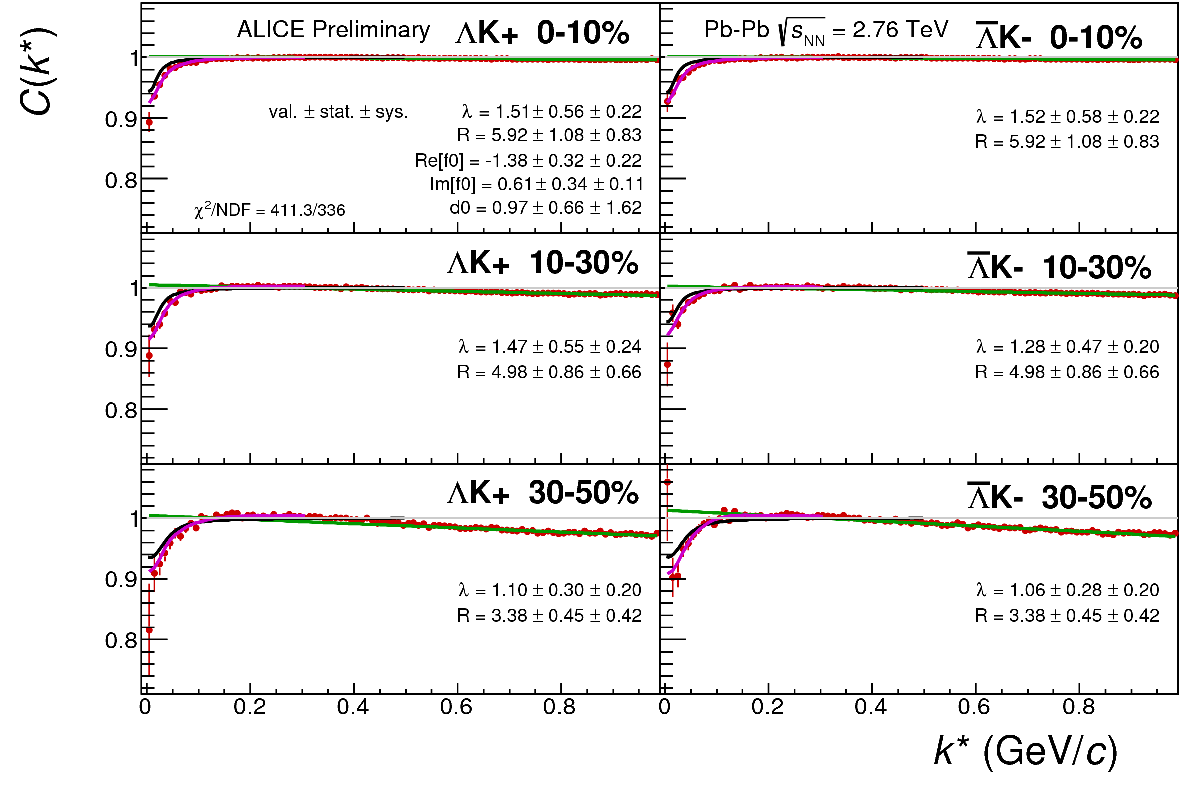
\includegraphics[width=\textwidth]{7_ResultsAndDiscussion/Figures/canKStarCfwFitsLamKchPwConj_0010_1030_3050UnZoomed_MomResCrctn_NonFlatBgdCrctn_10Res_PrimMaxDecay4fm_UsingXiDataAndCoulombOnly.pdf}
  \caption[$\Lambda$K$^{+}$($\bar{\Lambda}$K$^{-}$) Fits with 10 Residuals (Wide Range)]{Same as Fig. \ref{fig:LamKchPwConjFits_10Res}, but with a wider range of view.
Fits, with 10 residual correlations included, to the $\Lambda$K$^{+}$ (left) and $\bar{\Lambda}$K$^{-}$ (right) data for the centralities 0-10\% (top), 10-30\% (middle), and 30-50\% (bottom).
The lines represent the statistical errors, while the boxes represent the systematic errors.  
Each has unique $\lambda$ and normalization parameters.
The radii are shared amongst like centralities; the scattering parameters ($\mathbb{R}f_{0}$, $\mathbb{I}f_{0}$, $d_{0}$) are shared amongst all.
The black solid line represents the ``raw" fit, i.e. not corrected for momentum resolution effects nor non-flat background.  
The green line shows the fit to the non-flat background.
The purple points show the fit after momentum resolution and non-flat background corrections have been applied.
The initial values of the parameters is listed, as well as the final fit values with uncertainties.}
  \label{fig:LamKchPwConjFitsUnZoomed_10Res}
\end{figure}
\end{comment}



\begin{figure}[h]
  \centering
  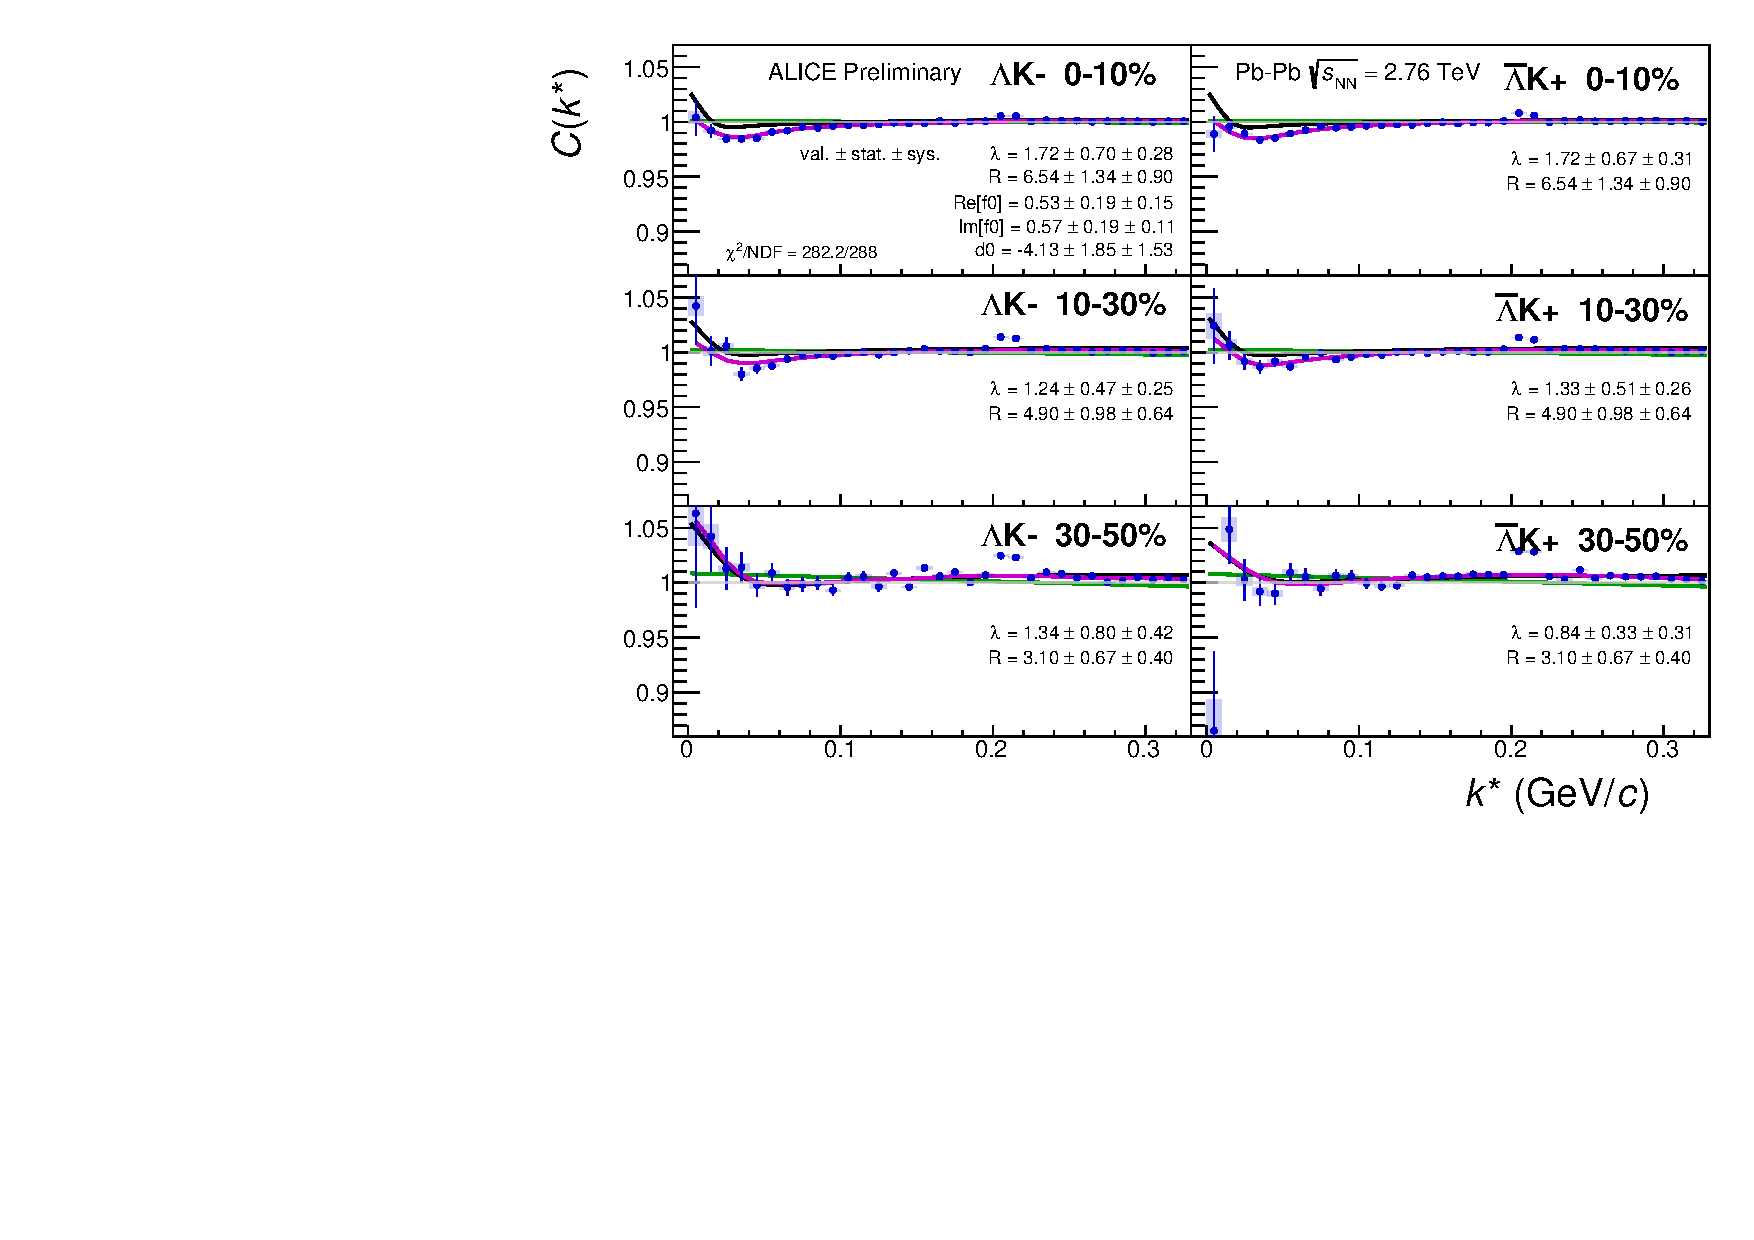
\includegraphics[width=\textwidth]{7_ResultsAndDiscussion/Figures/canKStarCfwFitsLamKchMwConj_0010_1030_3050_MomResCrctn_NonFlatBgdCrctn_10Res_PrimMaxDecay4fm_UsingXiDataAndCoulombOnly.pdf}
  \caption[$\Lambda$K$^{-}$($\bar{\Lambda}$K$^{+}$) Fits with 10 Residuals]{Fits, with 10 residual correlations included, to the $\Lambda$K$^{-}$(left) with $\bar{\Lambda}$K$^{+}$ (right) data for the centralities 0-10\% (top), 10-30\% (middle), and 30-50\% (bottom).
The lines represent the statistical errors, while the boxes represent the systematic errors.  
Each has unique $\lambda$ and normalization parameters.
The radii are shared amongst like centralities; the scattering parameters ($\mathbb{R}f_{0}$, $\mathbb{I}f_{0}$, $d_{0}$) are shared amongst all.
The black solid line represents the ``raw" fit, i.e. not corrected for momentum resolution effects nor non-flat background.  
The green line shows the fit to the non-flat background.
The purple points show the fit after momentum resolution and non-flat background corrections have been applied.
The initial values of the parameters is listed, as well as the final fit values with uncertainties.}
  \label{fig:LamKchMwConjFits_10Res}
\end{figure}

\begin{comment}
\begin{figure}[h]
  \centering
  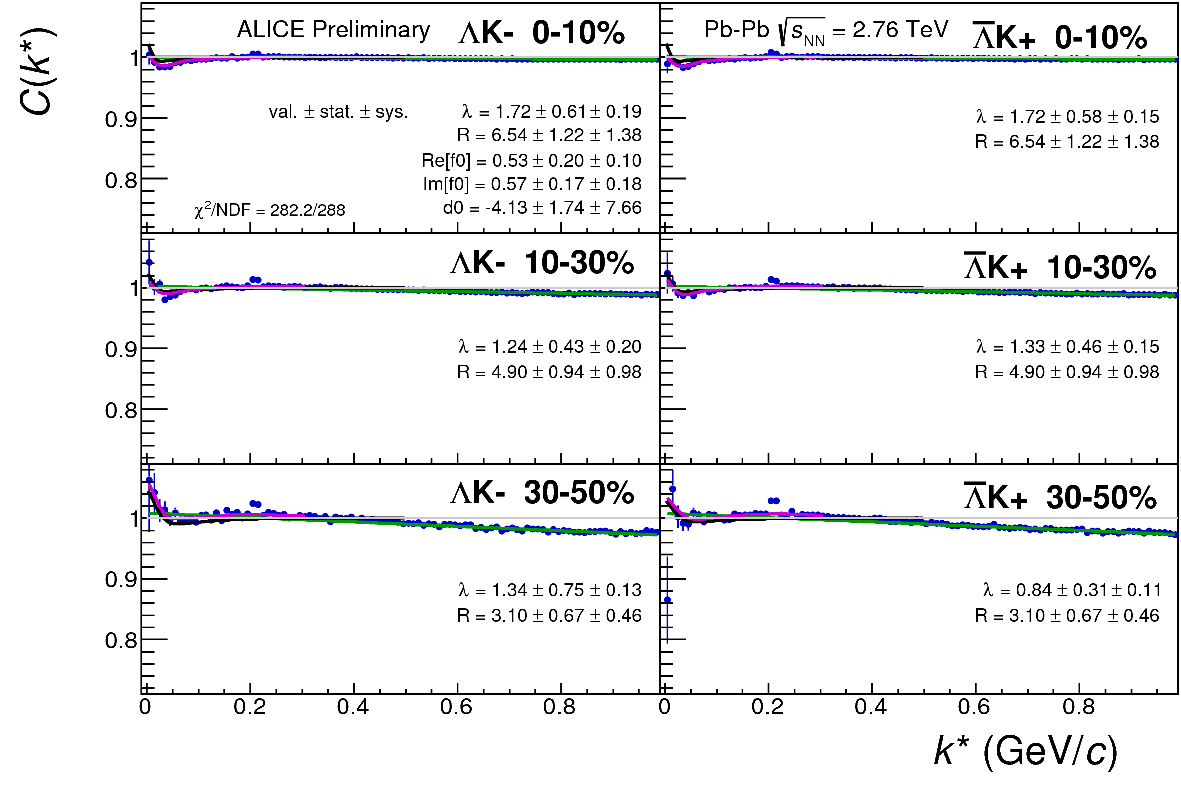
\includegraphics[width=\textwidth]{7_ResultsAndDiscussion/Figures/canKStarCfwFitsLamKchMwConj_0010_1030_3050UnZoomed_MomResCrctn_NonFlatBgdCrctn_10Res_PrimMaxDecay4fm_UsingXiDataAndCoulombOnly.pdf}
  \caption[$\Lambda$K$^{-}$($\bar{\Lambda}$K$^{+}$) Fits with 10 Residuals (Wide Range)]{Same as Fig. \ref{fig:LamKchMwConjFits_10Res}, but with a wider range of view.
Fits, with 10 residual correlations included, to the $\Lambda$K$^{-}$(left) with $\bar{\Lambda}$K$^{+}$ (right) data for the centralities 0-10\% (top), 10-30\% (middle), and 30-50\% (bottom).
The lines represent the statistical errors, while the boxes represent the systematic errors.  
Each has unique $\lambda$ and normalization parameters.
The radii are shared amongst like centralities; the scattering parameters ($\mathbb{R}f_{0}$, $\mathbb{I}f_{0}$, $d_{0}$) are shared amongst all.
The black solid line represents the ``raw" fit, i.e. not corrected for momentum resolution effects nor non-flat background.  
The green line shows the fit to the non-flat background.
The purple points show the fit after momentum resolution and non-flat background corrections have been applied.
The initial values of the parameters is listed, as well as the final fit values with uncertainties.}
  \label{fig:LamKchMwConjFitsUnZoomed_10Res}
\end{figure}
\end{comment}

\pagestyle{empty}
\begin{landscape}

\begin{table}[htbp]
 \centering
 \resizebox{\paperwidth}{!}{
 \begin{tabular}{|c|c|c|c|c|c|c|}
  \multicolumn{7}{c}{Fit Results $\Lambda$($\bar{\Lambda}$)K$^{0}_{S}$} \\
  \hline
  \multirow{3}{*}{Pair Type} & \multirow{3}{*}{Centrality} & \multicolumn{5}{c|}{Fit Parameters} \\
  \cline{3-7}
   & & $\lambda$ & $R$ & $\mathbb{R}f_{0}$ & $\mathbb{I}f_{0}$ & $d_{0}$ \\
  \hline  
  \multirow{3}{*}{$\Lambda$K$^{0}_{S}$}  
   &  0-10\% & \multirow{6}{*}{0.60 $\pm$ 0.63 (stat.) $\pm$ 0.17 (sys.)}  %Lambda
             & 2.94 $\pm$ 0.45 (stat.) $\pm$ 0.35 (sys.)  %Radius
             & \multirow{6}{*}{-0.40 $\pm$ 0.12 (stat.) $\pm$ 0.17 (sys.)}  %Ref0
             & \multirow{6}{*}{0.17 $\pm$ 0.08 (stat.) $\pm$ 0.12 (sys.)}  %Imf0
             & \multirow{6}{*}{1.94 $\pm$ 0.47 (stat.) $\pm$ 0.77 (sys.)} \\ %d0
             
   & 10-30\% & 
             & 2.39 $\pm$ 0.38 (stat.) $\pm$ 0.25 (sys.)  %Radius
             & & & \\
             
   & 30-50\% & 
             & 1.81 $\pm$ 0.29 (stat.) $\pm$ 0.12 (sys.)  %Radius
             & & & \\
  \cline{1-2}
  \cline{4-4}
  \multirow{3}{*}{$\bar{\Lambda}$K$^{0}_{S}$}  
   &  0-10\% & 
             & 2.94 $\pm$ 0.45 (stat.) $\pm$ 0.35 (sys.)  %Radius
             & & & \\
             
   & 10-30\% & 
             & 2.39 $\pm$ 0.38 (stat.) $\pm$ 0.25 (sys.)  %Radius
             & & & \\
             
   & 30-50\% & 
             & 1.81 $\pm$ 0.29 (stat.) $\pm$ 0.12 (sys.)  %Radius
             & & & \\
  \hline
 \end{tabular}}
 \caption{Fit Results $\Lambda$($\bar{\Lambda}$)K$^{0}_{S}$, with 10 residual correlations included. 
 Each pair is fit simultaneously with its conjugate (ie. $\Lambda$K$^{0}_{S}$ with $\bar{\Lambda}$K$^{0}_{S}$) across all centralities (0-10\%, 10-30\%, 30-50\%), for a total of 6 simultaneous analyses in the fit.
 Each analysis has a unique $\lambda$ and normalization parameter.
 The radii are shared between analyses of like centrality, as these should have similar source sizes.
 The scattering parameters ($\mathbb{R}f_{0}$, $\mathbb{I}f_{0}$, $d_{0}$) are shared amongst all.
 The fit is done on the data with only statistical error bars.
 The errors marked as ``stat." are those returned by MINUIT.
 The errors marked as ``sys." are those which result from my systematic analysis (as outlined in Section \ref{SystematicErrors}).}
 \label{tab:FitResultsLamK0_10Res}
\end{table}



%\end{landscape}
%\pagestyle{plain}

%\pagestyle{empty}
%\begin{landscape}

\begin{table}[htbp]
 \centering
 \resizebox{\paperwidth}{!}{
 \begin{tabular}{|c|c|c|c|c|c|c|}
  \multicolumn{7}{c}{Fit Results $\Lambda$($\bar{\Lambda}$)K$^{\pm}$} \\
  \hline
  \multirow{3}{*}{Pair Type} & \multirow{3}{*}{Centrality} & \multicolumn{5}{c|}{Fit Parameters} \\
  \cline{3-7}
   & & $\lambda$ & $R$ & $\mathbb{R}f_{0}$ & $\mathbb{I}f_{0}$ & $d_{0}$ \\
  \hline  
  \multirow{3}{*}{$\Lambda$K$^{+}$}  
   &  0-10\% & 1.51 $\pm$ 0.56 (stat.) $\pm$ 0.27 (sys.)  %Lambda
             & 5.92 $\pm$ 1.08 (stat.) $\pm$ 0.51 (sys.)  %Radius
             & \multirow{6}{*}{-1.38 $\pm$ 0.32 (stat.) $\pm$ 0.34 (sys.)}  %Ref0
             & \multirow{6}{*}{0.61 $\pm$ 0.34 (stat.) $\pm$ 0.20 (sys.)}  %Imf0
             & \multirow{6}{*}{0.97 $\pm$ 0.66 (stat.) $\pm$ 0.42 (sys.)} \\ %d0
             
   & 10-30\% & 1.47 $\pm$ 0.55 (stat.) $\pm$ 0.31 (sys.)  %Lambda
             & 4.98 $\pm$ 0.86 (stat.) $\pm$ 0.40 (sys.)  %Radius
             & & & \\
             
   & 30-50\% & 1.10 $\pm$ 0.30 (stat.) $\pm$ 0.27 (sys.)  %Lambda
             & 3.38 $\pm$ 0.45 (stat.) $\pm$ 0.28 (sys.)  %Radius
             & & & \\
  \cline{1-4}  
  \multirow{3}{*}{$\bar{\Lambda}$K$^{-}$}  
   &  0-10\% & 1.52 $\pm$ 0.58 (stat.) $\pm$ 0.33 (sys.)  %Lambda
             & 5.92 $\pm$ 1.08 (stat.) $\pm$ 0.51 (sys.)  %Radius
             & & & \\
             
   & 10-30\% & 1.28 $\pm$ 0.47 (stat.) $\pm$ 0.25 (sys.)  %Lambda
             & 4.98 $\pm$ 0.86 (stat.) $\pm$ 0.40 (sys.)  %Radius
             & & & \\
             
   & 30-50\% & 1.06 $\pm$ 0.28 (stat.) $\pm$ 0.16 (sys.)  %Lambda
             & 3.38 $\pm$ 0.45 (stat.) $\pm$ 0.28 (sys.)  %Radius
             & & & \\
  \hline
  \hline  
  \multirow{3}{*}{$\Lambda$K$^{-}$}  
   &  0-10\% & 1.72 $\pm$ 0.61 (stat.) $\pm$ 0.28 (sys.)  %Lambda
             & 6.54 $\pm$ 1.22 (stat.) $\pm$ 0.90 (sys.)  %Radius
             & \multirow{6}{*}{0.53 $\pm$ 0.20 (stat.) $\pm$ 0.15 (sys.)}  %Ref0
             & \multirow{6}{*}{0.57 $\pm$ 0.17 (stat.) $\pm$ 0.11 (sys.)}  %Imf0
             & \multirow{6}{*}{-4.13 $\pm$ 1.74 (stat.) $\pm$ 1.53 (sys.)} \\ %d0
             
   & 10-30\% & 1.24 $\pm$ 0.43 (stat.) $\pm$ 0.25 (sys.)  %Lambda
             & 4.90 $\pm$ 0.94 (stat.) $\pm$ 0.64 (sys.)  %Radius
             & & & \\
             
   & 30-50\% & 1.34 $\pm$ 0.75 (stat.) $\pm$ 0.42 (sys.)  %Lambda
             & 3.10 $\pm$ 0.67 (stat.) $\pm$ 0.40 (sys.)  %Radius
             & & & \\
  \cline{1-4}  
  \multirow{3}{*}{$\bar{\Lambda}$K$^{+}$}  
   &  0-10\% & 1.72 $\pm$ 0.58 (stat.) $\pm$ 0.31 (sys.)  %Lambda
             & 6.54 $\pm$ 1.22 (stat.) $\pm$ 0.90 (sys.)  %Radius
             & & & \\
             
   & 10-30\% & 1.33 $\pm$ 0.46 (stat.) $\pm$ 0.26 (sys.)  %Lambda
             & 4.90 $\pm$ 0.94 (stat.) $\pm$ 0.64 (sys.)  %Radius
             & & & \\
             
   & 30-50\% & 0.84 $\pm$ 0.31 (stat.) $\pm$ 0.31 (sys.)  %Lambda
             & 3.10 $\pm$ 0.67 (stat.) $\pm$ 0.40 (sys.)  %Radius
             & & & \\
  \hline
 \end{tabular}}
 \caption{Fit Results $\Lambda$($\bar{\Lambda}$)K$^{\pm}$, with 10 residual correlations included..
 Each pair is fit simultaneously with its conjugate (ie. $\Lambda$K$^{+}$ with $\bar{\Lambda}$K$^{-}$ and $\Lambda$K$^{-}$ with $\bar{\Lambda}$K$^{+}$) across all centralities (0-10\%, 10-30\%, 30-50\%), for a total of 6 simultaneous analyses in the fit.
 Each analysis has a unique $\lambda$ and normalization parameter.
 The radii are shared between analyses of like centrality, as these should have similar source sizes.
 The scattering parameters ($\mathbb{R}f_{0}$, $\mathbb{I}f_{0}$, $d_{0}$) are shared amongst all.
 The fit is done on the data with only statistical error bars.
 The errors marked as ``stat." are those returned by MINUIT.
 The errors marked as ``sys." are those which result from my systematic analysis (as outlined in Section \ref{SystematicErrors}).}
 \label{tab:FitResultsLamKch_10Res}
\end{table}


%%%%%%%%%%%%%%%%%%%%%%%%%%%%%%%%%%%%%%%%%%%%%%%%%%%%%%%%%%%%%%%%%%%%%%%%%%%%%%%%%%%%%%%%%%%%%
%%%%%%%%%%%%%%%%%% QM 17 Stuff %%%%%%%%%%%%%%%%%%%%%%%%%%%%%%%%%%%%%%%%%%%%%%%%%%%%%%%%%%%%%%

\clearpage
\begin{table}[htbp]
 \centering
 \resizebox{\paperwidth}{!}{
 \begin{tabular}{|c|c|c|c|c|}
  \multicolumn{2}{c}{} & \multicolumn{3}{c}{\textbf{\large Fit Parameters} (\large \textbf{value $\pm$ statistical error $\pm$ systematic error)}} \\
  \hline
  \textbf{\large Pair Type} & \textbf{\large Centrality} & \multicolumn{3}{c|}{\textbf{\large R}} \\
  \cline{1-5}
  \multirow{5}{*}{\large \textbf{$\Lambda$K$^{+}$ \& $\bar{\Lambda}$K$^{-}$}}
  &  \textbf{0-10\%} & \multicolumn{3}{c|}{\textbf{5.92 $\pm$ 1.08 $\pm$ 0.51}} \\  %Radius
  & \textbf{10-30\%} & \multicolumn{3}{c|}{\textbf{4.98 $\pm$ 0.86 $\pm$ 0.40}} \\  %Radius
  & \textbf{30-50\%} & \multicolumn{3}{c|}{\textbf{3.38 $\pm$ 0.45 $\pm$ 0.28}} \\  %Radius
  \cline{2-5}
  & & \large $\mathbf{\Re f_{0}}$ & \large $\mathbf{\Im f_{0}}$ & \large $\mathbf{d_{0}}$ \\
  \cline{3-5}  
  & & \textbf{-1.38 $\pm$ 0.32 $\pm$ 0.34} & \textbf{0.61 $\pm$ 0.34 $\pm$ 0.20} & \textbf{0.97 $\pm$ 0.66 $\pm$ 0.42} \\
  
  \hline
  \hline
  
  \multirow{5}{*}{\large \textbf{$\Lambda$K$^{-}$ \& $\bar{\Lambda}$K$^{+}$}} 
  &  \textbf{0-10\%} & \multicolumn{3}{c|}{\textbf{6.54 $\pm$ 1.22 $\pm$ 0.90}} \\  %Radius
  & \textbf{10-30\%} & \multicolumn{3}{c|}{\textbf{4.90 $\pm$ 0.94 $\pm$ 0.64}} \\  %Radius
  & \textbf{30-50\%} & \multicolumn{3}{c|}{\textbf{3.10 $\pm$ 0.67 $\pm$ 0.40}} \\  %Radius
  \cline{2-5}
  & & \large $\mathbf{\Re f_{0}}$ & \large $\mathbf{\Im f_{0}}$ & \large $\mathbf{d_{0}}$ \\
  \cline{3-5}     
  & & \textbf{0.53 $\pm$ 0.20 $\pm$ 0.15} & \textbf{0.57 $\pm$ 0.17 $\pm$ 0.11} & \textbf{-4.13 $\pm$ 1.74 $\pm$ 1.53} \\
   
  \hline
  \hline  
  
  \multirow{5}{*}{\large \textbf{$\Lambda$K$^{0}_{S}$ \& $\bar{\Lambda}$K$^{0}_{S}$}}  
   &  \textbf{0-10\%} & \multicolumn{3}{c|}{\textbf{2.94 $\pm$ 0.45 $\pm$ 0.35}} \\  %Radius
   & \textbf{10-30\%} & \multicolumn{3}{c|}{\textbf{2.39 $\pm$ 0.38 $\pm$ 0.25}} \\  %Radius
   & \textbf{30-50\%} & \multicolumn{3}{c|}{\textbf{1.81 $\pm$ 0.29 $\pm$ 0.12}} \\  %Radius
   \cline{2-5}   
   & & \large $\mathbf{\Re f_{0}}$ & \large $\mathbf{\Im f_{0}}$ & \large $\mathbf{d_{0}}$ \\
   \cline{3-5} 
   & & \textbf{-0.40 $\pm$ 0.12 $\pm$ 0.17} & \textbf{0.17 $\pm$ 0.08 $\pm$ 0.12} & \textbf{1.94 $\pm$ 0.47 $\pm$ 0.77} \\
  \hline
 \end{tabular}}
 \caption{Fit Results $\Lambda$($\bar{\Lambda}$)K$^{\pm}$ and $\Lambda$($\bar{\Lambda}$)K$^{0}_{\mathrm{S}}$, with 10 residual correlations included. ($\lambda$ parameters not shown).  This table is a condensed version of Tables \ref{tab:FitResultsLamK0_10Res} and \ref{tab:FitResultsLamKch_10Res}} 
 \label{tab:FitResultsLamKCondensed_10Res}
\end{table}

\end{landscape}
\pagestyle{plain}

\begin{figure}[h]
  \centering
  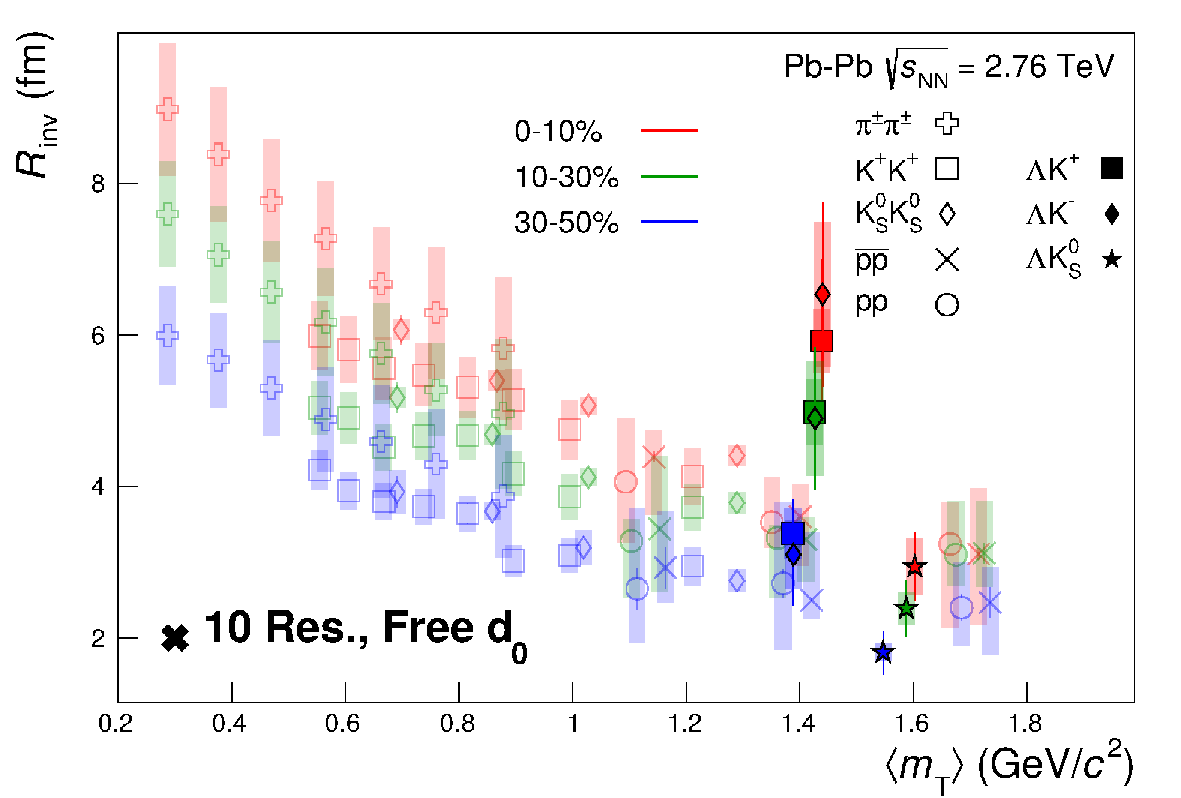
\includegraphics[width=\textwidth]{7_ResultsAndDiscussion/Figures/mTscaling_MinvCalc_OutlinedPoints_OthersTransparent_10Res_FreeD0.pdf}
  \caption[$m_{\mathrm{T}}$ Scaling of Radii: 10 Residuals in Fit]{10 residual correlations in $\Lambda$K fits.  Extracted fit $R_{\mathrm{inv}}$ parameters as a function of pair transverse mass ($m_{\mathrm{T}}$) for various pair systems over several centralities. The ALICE published data \cite{Adam:2015vja} is shown with transparent, open symbols.  The new $\Lambda$K results are shown with opaque, filled symbols.  In the left, the $\Lambda$K$^{+}$ (with it's conjugate pair) results are shown separately from the $\Lambda$K$^{-}$ (with it's conjugate pair) results.  In the right, all $\Lambda$K$^{\pm}$ results are averaged.}
  \label{fig:mTScalingOfRadii}
\end{figure}

\clearpage

\end{document}